%!TEX root = ../ENTRUST_TR.tex

\textit{Runtime quantitative verification} (RQV) \cite{Calinescu2012:ACM} is an approach to implementing the closed control loop of self-adaptive systems in which the adaptation decisions are driven by the continual verification of stochastic models. RQV was introduced in \cite{Calinescu2009:ICSE,Epifani2009:ICSE} and further refined in \cite{Calinescu2011:TSE,Filieri2011:ICSE,Johnson2013:CBSE}. 


Figure~\ref{fig:RQV} depicts the adaptation workflow of an RQV-based self-adaptive system. The approach involves monitoring the system (e.g., the UUV) and its environment continuously, to identify relevant changes and quantify them using fast on-line learning techniques. When these changes are significant and/or periodically, an RQV step is triggered, to identify which scenario the system operates in, and to select the associated model from a family of system models (i.e., a \emph{parametric model}) that correspond to different such scenarios. The selected model is then analysed using quantitative verification, to identify and/or predict violations of QoS requirements such as response time, availability and cost. When QoS violations are identified or predicted, the verification results support the selection of a new set of values for the configurable system parameters, so that enforcing this new configuration is \emph{guaranteed} to restore or maintain compliance with QoS requirements, respectively.

\begin{figure}[t]
\centering
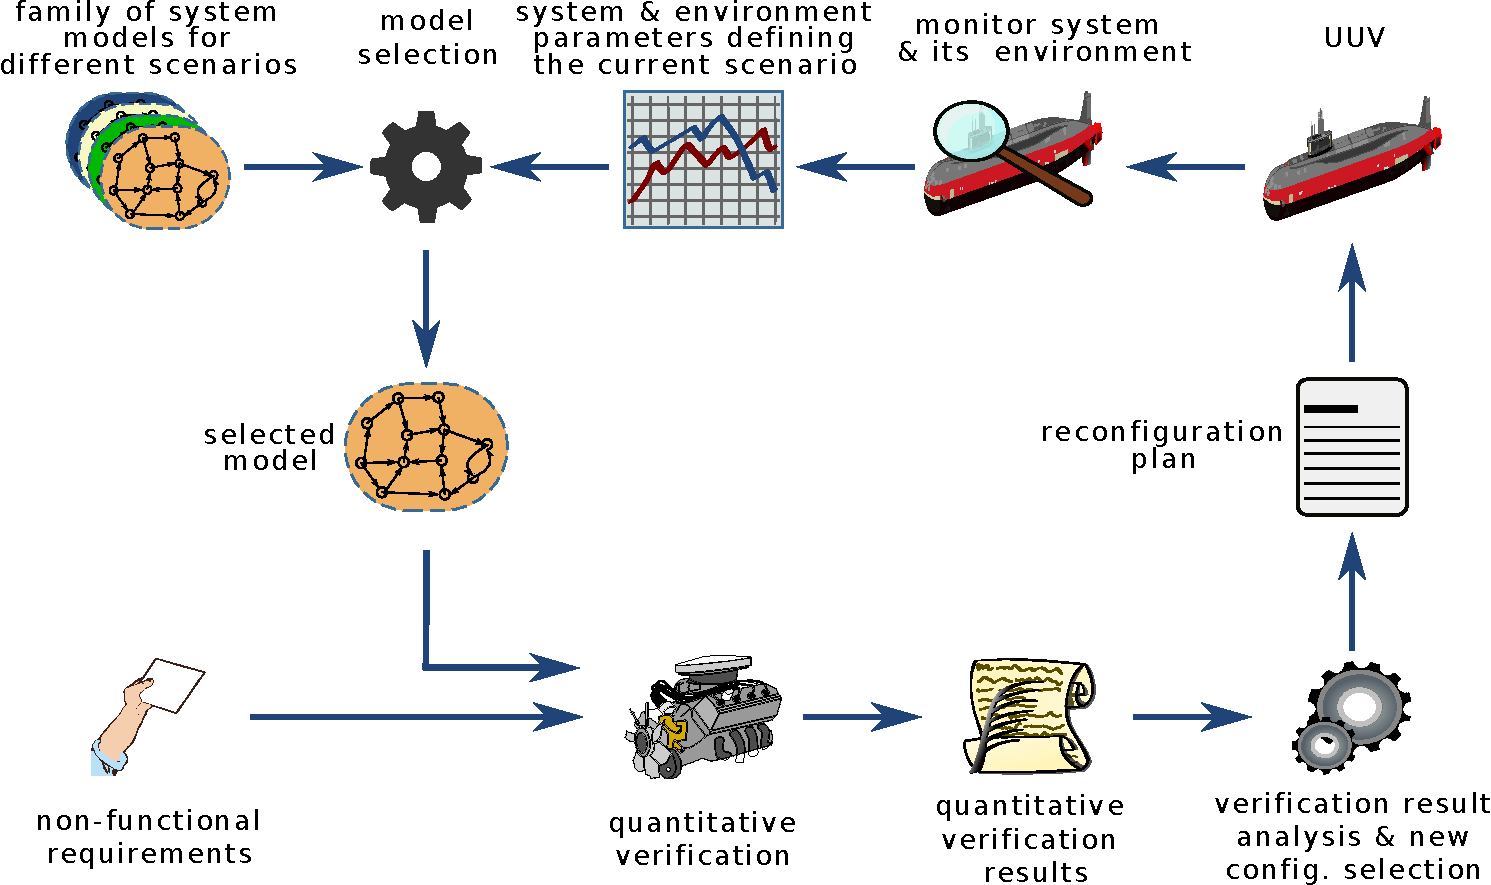
\includegraphics[width=0.75\hsize]{figures/rqv.pdf}
\caption{RQV-based self-adaptive system}
\label{fig:RQV}

\vspace*{-2mm}
\end{figure}